% Number 650
% GM 2D Algebra Units
% g on another planet; 2D
% JG

% Watermark
\AddToShipoutPicture*{\BackgroundPic}

\addtocounter {ProbNum} {1}

%\begin{floatingfigure}[r]{.2\textwidth}
%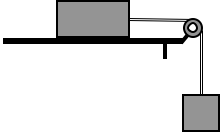
\includegraphics[scale=.6]{/Users/jgates/desktop/latex/pics/halfatwood3}
%\end{floatingfigure}
 
{\bf \Large{\arabic{ProbNum}}} You take a trip to a round asteroid.  It has the same average density as the Earth, but is only 650 km in radius. 
 
\bigskip
What is the freefall acceleration on the surface of this asteroid?\paragraph{}
\noindent
\vfill

If you could kick a soccer ball a maximum distance of 34 meters back on Earth, how far could you kick it here?
\vfill
%\hfill 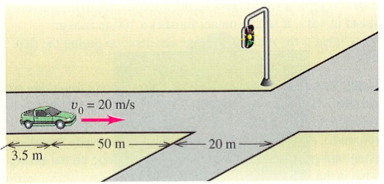
\includegraphics[scale=.85]{/Users/jgates/desktop/latex/pics/redlight.png}
\newpage
